\documentclass{article}
\usepackage{float}
\usepackage{adjustbox}
\usepackage{graphicx}

\begin{document}
	\title{R\'esum\'e}
	\author{Rishabh Talreja}
	\maketitle
	Name : Rishabh Talreja\\
   	Address:101,First Floor Hari apartments, College Road Belgaum,Karnataka,590001\\
   	Contact Number:9916535881\\
   	E-mail id:rishabh16398@gmail.com
		\begin{figure}[h]
		\hspace{10cm}
		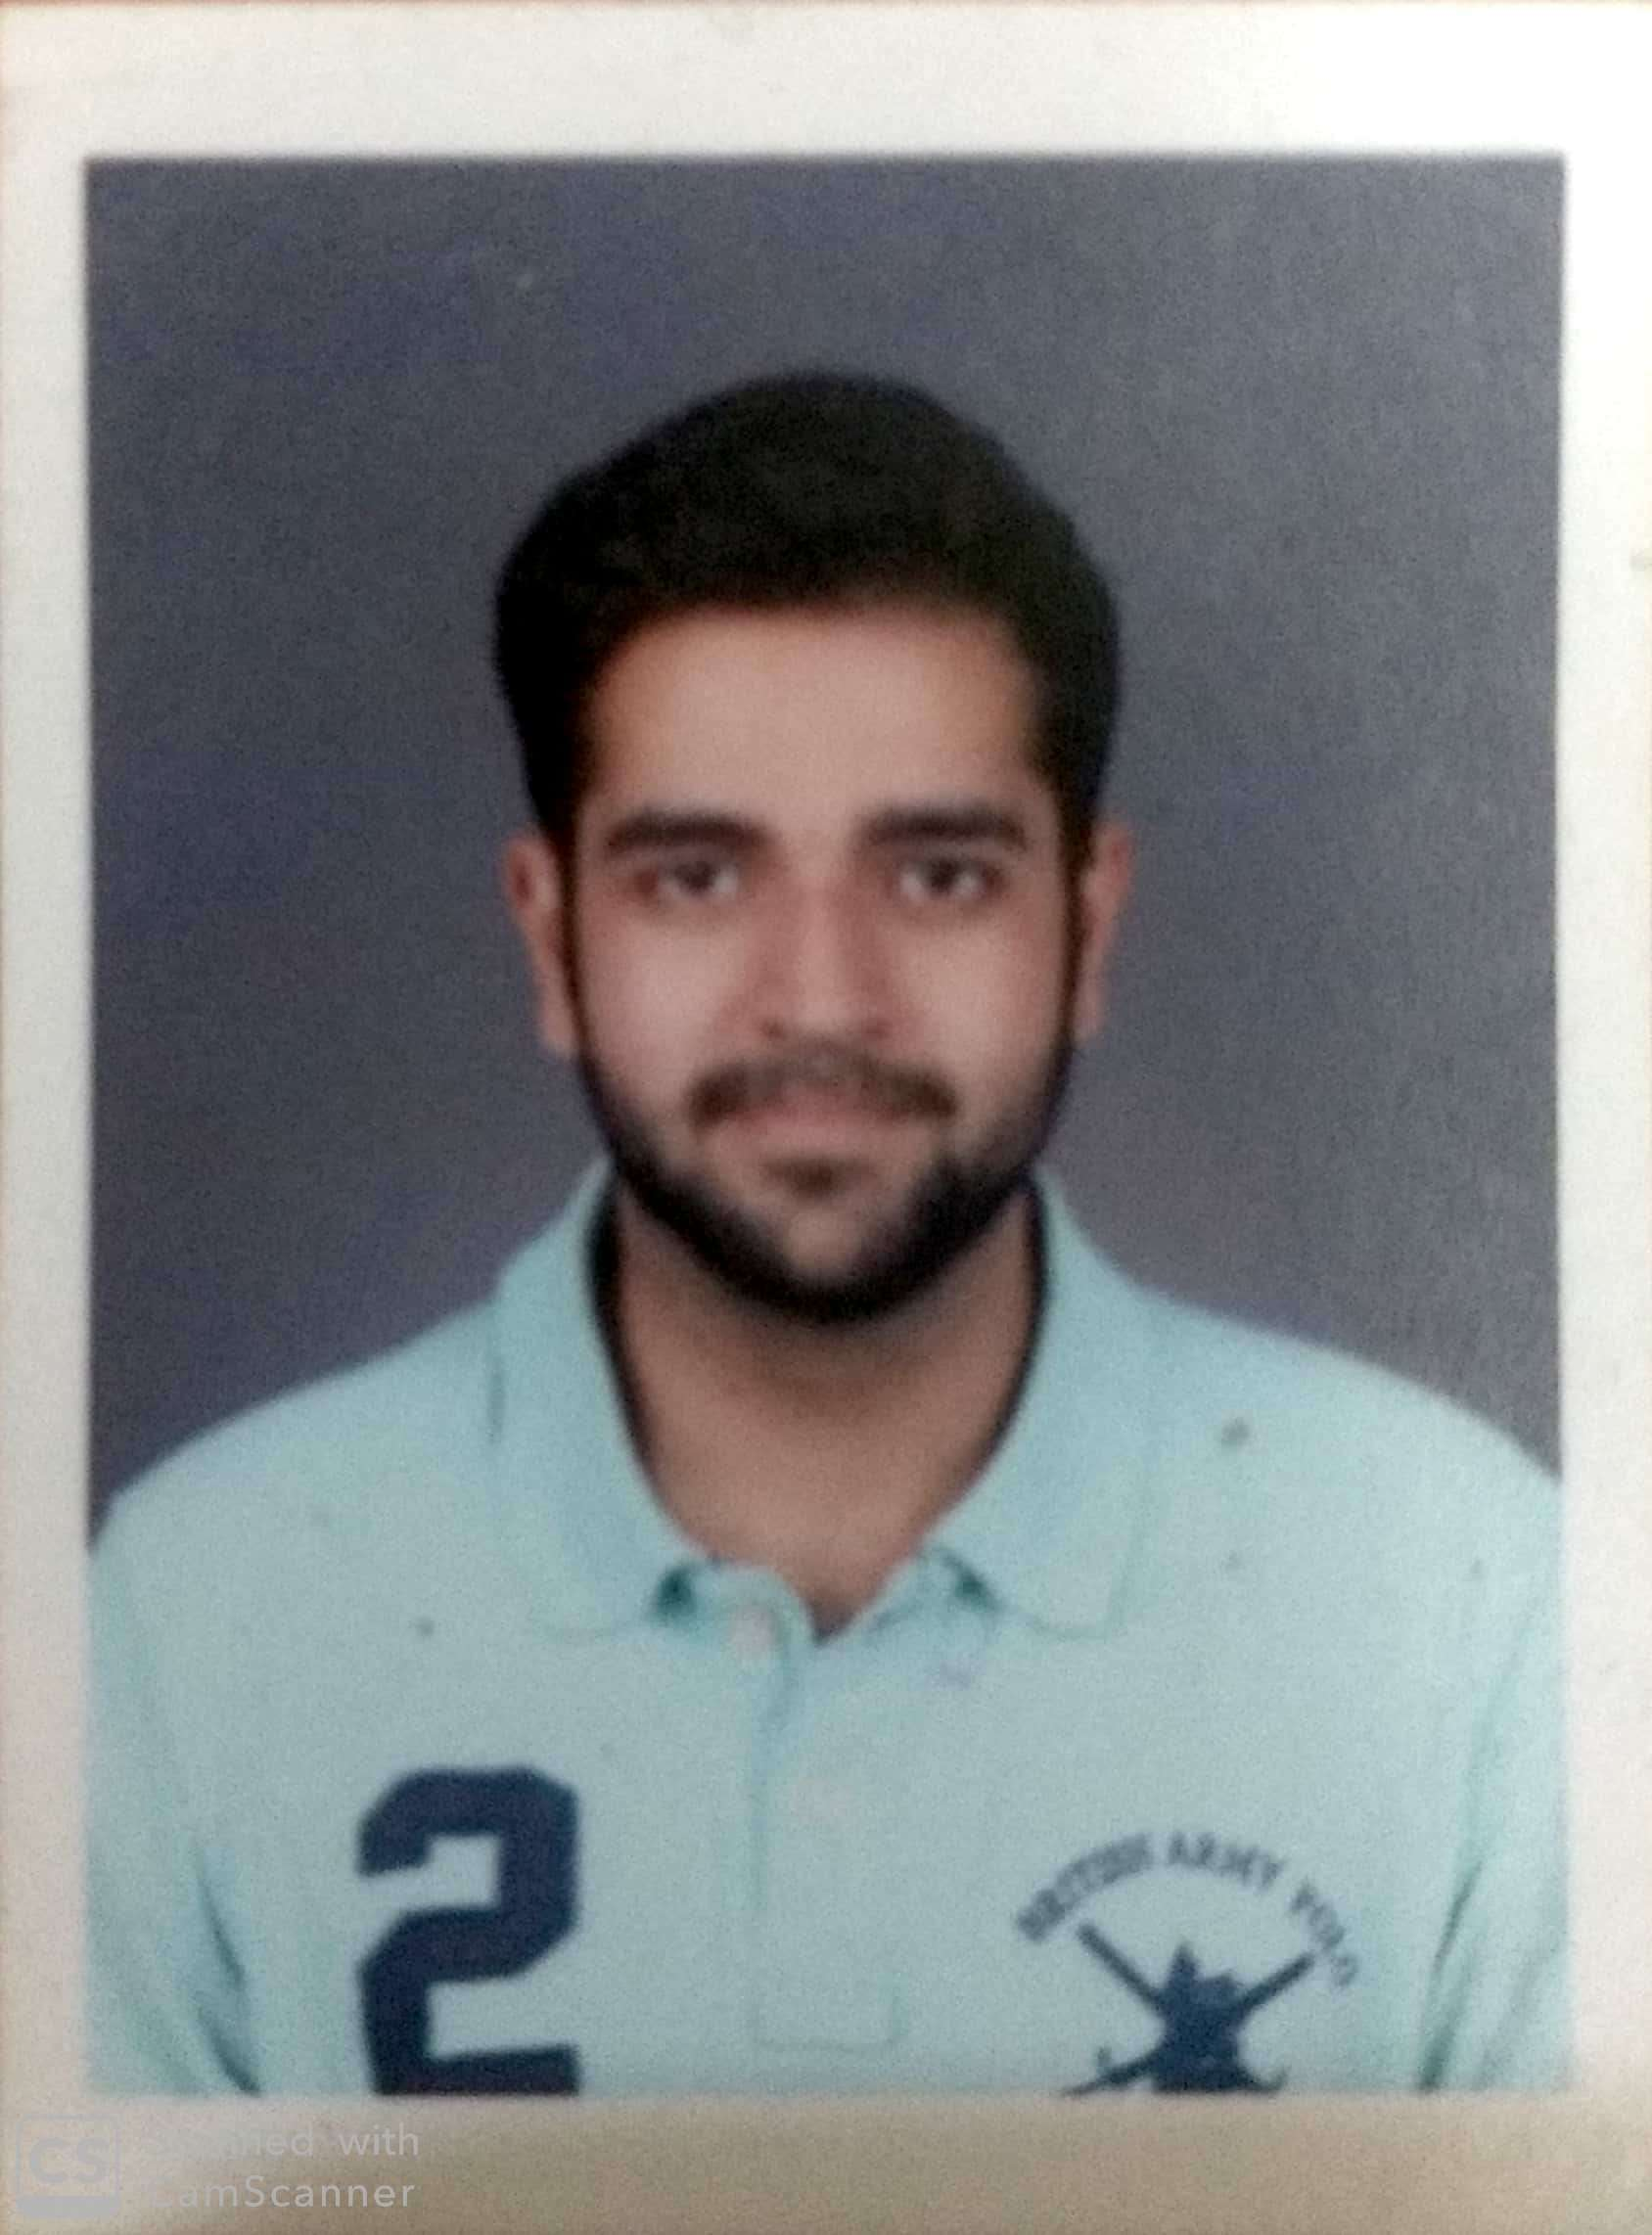
\includegraphics[height=5cm]{pic.jpg}
	\end{figure}
	\section{Career Objectives}
To keep updating my skills based on the changing technical environment. To focus on problem
solving for making a better future. To contribute towards the development of the country.
	\section{Education}
{
	\begin{table}[h]
		\begin{adjustbox}{max width=470pt}
			\begin{tabular}{|p{4cm}|l |l| p{3cm}|l| l| p{1cm} | l||}
				\hline
				\rule{0pt}{4ex}
				\textbf{Degree} & \textbf{College/School} & \textbf{University/Board} & \textbf{Passing Year} & \textbf{Pass Percentage} \\
				\hline
				\rule{0pt}{4ex}
				10th & Kendriya Vidyalaya No 2 & Central Board Of Secondary Education & 2014 & 9.8 CGPA\\
				\hline
				\rule{0pt}{4ex}
				12th & Kendriya Vidyalaya No 2 & Central Board Of Secondary Education & 2016 & 86.7 \% \\
				\hline
				\rule{0pt}{4ex}
				B.E(Computer Science and Engineering) & Jain College Of Engineering & 
				Visvesvaraya
				Technological
				University 
				& 2020 & 8.5 CGPA\\
				\hline
			\end{tabular}
		\end{adjustbox}
	\end{table}
}
	\section{Projects}
		\subsection{Website Development in Flask}
			A web-based portal for managing employees. 
			\begin{itemize}
				\item Programming languages/Markup Language used: HTML, CSS, Bootstrap v3.3.7, Python.
				\item Tools used: Atom text editor, Apache Server, PostgreSQL, GitHub. 
			\end{itemize}
		\subsection{E-Yantra 2018-2019}
			Build a line following robot with a lifting mechanism and a lift.
			\begin{itemize}
				\item Language used: Embedded C. 
				\item Tools used: Atmel Studio, Vrep.
			\end{itemize}
		\subsection{Game Development}
			\begin{itemize}
				\item Language used: C\#. 
				\item Tools used: Unity Engine, Visual Studios. 
			\end{itemize}
		\subsection{Fully Functional E-commerce website}
			A Web application developed in PHP for buying products online
			\begin{itemize}
				\item  Used:PHP, SQL,HTML,CSS.
				\item Tools used: MySQL, WAMP Server, Sublime Text Editor 
			\end{itemize} 
		\subsection{College Fest Website}
			Developed a website for college fest.
	\section{Training \& Internships}
			\subsection{Python Developer at Shrestha IT}
			Worked at Shrestha IT as an intern for 2 months.There I worked on bash script in Linux and developed website using FLASK. 
			\subsection{Internee at Shivani Enterprises}
			Currently working as an intern at Shivani enterprises.Working on Workfusion RPA express.
	\section{Technical Skills}
			\subsection{Programming Languages known:}
			\begin{itemize}
				\item C
				\item C++
				\item C\#
				\item JAVA
				\item Python
				\item Embedded C
				\item PHP
			\end{itemize}
			\subsection{Markup Languages known:}\
			\begin{itemize}
				\item HTML
				\item TeX
			\end{itemize}
			\subsection{Database:}
			\begin{itemize}
				\item PostgreSQL
				\item MySQL
			\end{itemize}
		\section{Soft Skills}
		\begin{itemize}
			\item Good communication skills
			\item Leadership quality
			\item Problem solving ability
			\item Ability to Work Under Pressure and Time Management
		\end{itemize}
		\section{Extra Curricular Activities}
			\begin{itemize}
				\item Student head of National Service Scheme(NSS)
				\item Student coordinator of the CSE department in the college
				\item Director of International Service at the Rotaract Club of Venugram.
				\item Was the School Captain .
				\item Part of college debate team.
				\item Rhythm guitarist for a band name Yagna.
			\end{itemize}
		\section{Co-Curricular Activities}
			\begin{itemize}
				\item Game Design and animation
				\item Competitive Coding 
			\end{itemize}
			
\end{document}

